% !TeX spellcheck = es_AR
\documentclass[10pt, a4paper]{article}

\usepackage{caratula}

\usepackage[utf8]{inputenc}
\usepackage[spanish]{babel} % separación silábica en castellano

%\usepackage[paper=a4paper, margin=2cm]{geometry} % especifico márgenes manualmente
\usepackage{a4wide} % margenes un poco más anchos

%\usepackage{caratula/caratula}
%\graphicspath{ {images/} }
%\usepackage{tikz}
%\usepackage{tikz-qtree}
%\usepackage{framed}
%\usepackage{array}
%\usepackage{tabular}

\usepackage{microtype} % saca warnings de underfull boxes
\usepackage{fancyhdr} % encabezado y pie de página
\usepackage{lastpage} % para que muestre la última página en footer

% Comandos para figuras, graficos, tikz, etc.
\usepackage{tikz}
\usepackage{epsfig}
\usepackage{graphicx}
\usepackage{epsfig}
\usepackage{caption}
\usepackage{subcaption}
\usepackage{svg}

% Comandos para teoremas, etc.
\usepackage{amsmath}
\usepackage{amsthm}
\usepackage{amssymb}

% comandos para algoritmos
\usepackage{algorithm}
\usepackage[noend]{algpseudocode}
\algnewcommand{\IfThenElse}[3]{% \IfThenElse{<if>}{<then>}{<else>}
\State \algorithmicif\ #1\ \algorithmicthen\ #2\ \algorithmicelse\ #3}
\algnewcommand{\IfThen}[2]{% \IfThenElse{<if>}{<then>}
  \State \algorithmicif\ #1\ \algorithmicthen\ #2}
  
\newcommand{\norm}[1]{\left\lVert#1\right\rVert_2}
\usepackage{hyperref}
\usepackage{siunitx}

\pagestyle{fancy} % Acomodo el encabezado y pie de página.
\lhead{Fundamentos de la Computación Gráfica}
\setlength{\headheight}{12pt}
\rhead{Segundo Cuatrimestre 2021}
\cfoot{\thepage /\pageref{LastPage}}

\begin{document}

% **************************************************************************
%
%  Package 'caratula', version 0.5 (para componer caratulas de TPs del DC).
%
%  En caso de dudas, problemas o sugerencias sobre este package escribir a
%  Brian J. Cardiff (bcardif arroba gmail.com).
%  Nico Rosner (nrosner arroba dc.uba.ar).
%
% **************************************************************************

% ----- Informacion sobre el package para el sistema -----------------------

\NeedsTeXFormat{LaTeX2e}
\ProvidesPackage{caratula}[2013/08/04 v0.5 Para componer caratulas de TPs del DC]
\RequirePackage{ifthen}
\usepackage[pdftex]{graphicx}

% ----- Imprimir un mensajito al procesar un .tex que use este package -----

\typeout{Cargando package 'caratula' v0.5 (2013/08/04)}

% ----- Algunas variables --------------------------------------------------

\let\Materia\relax
\let\Submateria\relax
\let\Titulo\relax
\let\Subtitulo\relax
\let\Grupo\relax
\let\Fecha\relax
\let\Logoimagefile\relax
\newcommand{\LabelIntegrantes}{}
\newboolean{showLU}
\newboolean{showEntregas}
\newboolean{showDirectores}
\newboolean{showCoDirectores}

% ----- Comandos para que el usuario defina las variables ------------------

\def\materia#1{\def\Materia{#1}}
\def\submateria#1{\def\Submateria{#1}}
\def\titulo#1{\def\Titulo{#1}}
\def\subtitulo#1{\def\Subtitulo{#1}}
\def\grupo#1{\def\Grupo{#1}}
\def\fecha#1{\def\Fecha{#1}}
\def\logoimagefile#1{\def\Logoimagefile{#1}}

% ----- Token list para los integrantes ------------------------------------

\newtoks\intlist\intlist={}

\newtoks\intlistSinLU\intlistSinLU={}

\newcounter{integrantesCount}
\setcounter{integrantesCount}{2}
\newtoks\intTabNombre\intTabNombre={}
\newtoks\intTabLU\intTabLU={}
\newtoks\intTabEmail\intTabEmail={}

\newcounter{directoresCount}
\setcounter{directoresCount}{0}
\newtoks\direcTabNombre\direcTabNombre={}
\newtoks\direcTabEmail\direcTabEmail={}

\newcounter{coDirectoresCount}
\setcounter{coDirectoresCount}{0}
\newtoks\codirecTabNombre\codirecTabNombre={}
\newtoks\codirecTabEmail\codirecTabEmail={}


% ----- Comando para que el usuario agregue integrantes --------------------

\def\integrante#1#2#3{%
    \intlist=\expandafter{\the\intlist\rule{0pt}{1.2em}#1&#2&\tt #3\\[0.2em]}%
    \intlistSinLU=\expandafter{\the\intlistSinLU\rule{0pt}{1.2em}#1 & \tt #3\\[0.2em]}%
    %
    \ifthenelse{\value{integrantesCount} > 0}{%
        \intTabNombre=\expandafter{\the\intTabNombre & #1}%
        \intTabLU=\expandafter{\the\intTabLU & #2}%
        \intTabEmail=\expandafter{\the\intTabEmail & \tt #3}%
    }{
        \intTabNombre=\expandafter{\the\intTabNombre #1}%
        \intTabLU=\expandafter{\the\intTabLU #2}%
        \intTabEmail=\expandafter{\the\intTabEmail \tt #3}%
    }%
    \addtocounter{integrantesCount}{1}%
}

\def\director#1#2{%
    \ifthenelse{\value{directoresCount} > 0}{%
        \direcTabNombre=\expandafter{\the\direcTabNombre & #1}%
        \direcTabEmail=\expandafter{\the\direcTabEmail & \tt #2}%
    }{
        \direcTabNombre=\expandafter{\the\direcTabNombre #1}%
        \direcTabEmail=\expandafter{\the\direcTabEmail \tt #2}%
    }%
    \addtocounter{directoresCount}{1}%
}

\def\codirector#1#2{%
    \ifthenelse{\value{coDirectoresCount} > 0}{%
        \codirecTabNombre=\expandafter{\the\codirecTabNombre & #1}%
        \codirecTabEmail=\expandafter{\the\codirecTabEmail & \tt #2}%
    }{
        \codirecTabNombre=\expandafter{\the\codirecTabNombre #1}%
        \codirecTabEmail=\expandafter{\the\codirecTabEmail \tt #2}%
    }%
    \addtocounter{coDirectoresCount}{1}%
}


% ----- Macro para generar la tabla de integrantes -------------------------

\newcommand{\tablaIntegrantes}{\ }

\newcommand{\tablaIntegrantesVertical}{%
\ifthenelse{\boolean{showLU}}{%
    \begin{tabular}[t]{| l @{\hspace{4ex}} c @{\hspace{4ex}} l|}
        \hline
        \multicolumn{1}{|c}{\rule{0pt}{1.2em} \LabelIntegrantes} & LU &  \multicolumn{1}{c|}{Correo electr\'onico} \\[0.2em]
        \hline \hline
        \the\intlist
        \hline
    \end{tabular}
}{
    \begin{tabular}[t]{| l @{\hspace{4ex}} @{\hspace{4ex}} l|}
        \hline
        \multicolumn{1}{|c}{\rule{0pt}{1.2em} \LabelIntegrantes} &  \multicolumn{1}{c|}{Correo electr\'onico} \\[0.2em]
        \hline \hline
        \the\intlistSinLU
        \hline
    \end{tabular}
    }%
}

\newcommand{\tablaIntegrantesHorizontal}{%
    \begin{tabular}[t]{ *{\value{integrantesCount}}{c} }
    \the\intTabNombre \\%
\ifthenelse{\boolean{showLU}}{
    \the\intTabLU \\%
}{}
    \the\intTabEmail %
    \end{tabular}%
}

\newcommand{\tablaDirectores}{%
\ifthenelse{\boolean{showDirectores}}{%
	\bigskip
	Directores

	\smallskip
    \begin{tabular}[t]{ *{\value{directoresCount}}{c} }
    \the\direcTabNombre \\%
    \the\direcTabEmail %
    \end{tabular}%
}{}%
}

\newcommand{\tablaCoDirectores}{%
\ifthenelse{\boolean{showCoDirectores}}{%
	\bigskip
	Co-Directores

	\smallskip
    \begin{tabular}[t]{ *{\value{coDirectoresCount}}{c} }
    \the\codirecTabNombre \\%
    \the\codirecTabEmail %
    \end{tabular}%
}{}%
}

\newcommand{\tablaEntregas}{%
\ifthenelse{\boolean{showEntregas}}{%
  \bigskip%
  \begin{tabular}[t]{|l p{3.5cm} p{1.5cm}|}%
  \hline%
  \rule{0pt}{1.2em} Instancia & Docente & Nota \\[0.2em] %
  \hline%
  \hline%
  \rule{0pt}{1.2em} Primera entrega & & \\[0.2em] %
  \hline%
  \rule{0pt}{1.2em} Segunda entrega & & \\[0.2em] %
  \hline%
  \end{tabular}%
}{}%
}

% ----- Codigo para manejo de errores --------------------------------------

\def\se{\let\ifsetuperror\iftrue}
\def\ifsetuperror{%
    \let\ifsetuperror\iffalse
    \ifx\Materia\relax\se\errhelp={Te olvidaste de proveer una \materia{}.}\fi
    \ifx\Titulo\relax\se\errhelp={Te olvidaste de proveer un \titulo{}.}\fi
    \edef\mlist{\the\intlist}\ifx\mlist\empty\se%
    \errhelp={Tenes que proveer al menos un \integrante{nombre}{lu}{email}.}\fi
    \expandafter\ifsetuperror}

\def\aftermaketitle{%
  \setcounter{page}{1}
}

% ----- \maketitletxt correspondiente a la versión v0.2.1 (texto v0.2 + fecha ) ---------

\def\maketitletxt{%
    \ifsetuperror\errmessage{Faltan datos de la caratula! Ingresar 'h' para mas informacion.}\fi
    \thispagestyle{empty}
    \begin{center}
    \vspace*{\stretch{2}}
    {\LARGE\textbf{\Materia}}\\[1em]
    \ifx\Submateria\relax\else{\Large \Submateria}\\[0.5em]\fi
    \ifx\Fecha\relax\else{\Large \Fecha}\\[0.5em]\fi
    \par\vspace{\stretch{1}}
    {\large Departamento de Computaci\'on}\\[0.5em]
    {\large Facultad de Ciencias Exactas y Naturales}\\[0.5em]
    {\large Universidad de Buenos Aires}
    \par\vspace{\stretch{3}}
    {\Large \textbf{\Titulo}}\\[0.8em]
    {\Large \Subtitulo}
    \par\vspace{\stretch{3}}
    \ifx\Grupo\relax\else\textbf{\Grupo}\par\bigskip\fi
    \tablaIntegrantes
    \end{center}
    \vspace*{\stretch{3}}
    \newpage\aftermaketitle}

% ----- \maketitletxtlogo correspondiente v0.2.1 (texto con fecha y logo) ---------

\def\maketitletxtlogo{%
    \ifsetuperror\errmessage{Faltan datos de la caratula! Ingresar 'h' para mas informacion.}\fi
    \thispagestyle{empty}
    \begin{center}
    \ifx\Logoimagefile\relax\else\includegraphics{\Logoimagefile}\fi \hfill 
\includegraphics{imgs/logo_dc}\\[1em]
    \vspace*{\stretch{2}}
    {\LARGE\textbf{\Materia}}\\[1em]
    \ifx\Submateria\relax\else{\Large \Submateria}\\[0.5em]\fi
    \ifx\Fecha\relax\else{\large \Fecha}\\[0.5em]\fi
    \par\vspace{\stretch{1}}
    {\large Departamento de Computaci\'on}\\[0.5em]
    {\large Facultad de Ciencias Exactas y Naturales}\\[0.5em]
    {\large Universidad de Buenos Aires}
    \par\vspace{\stretch{3}}
    {\Large \textbf{\Titulo}}\\[0.8em]
    {\Large \Subtitulo}
    \par\vspace{\stretch{3}}
    \ifx\Grupo\relax\else\textbf{\Grupo}\par\bigskip\fi
    \tablaIntegrantes
    \end{center}
    \vspace*{\stretch{4}}
    \newpage\aftermaketitle}

% ----- \maketitlegraf correspondiente a la versión v0.3 (gráfica) -------------

\def\maketitlegraf{%
    \ifsetuperror\errmessage{Faltan datos de la caratula! Ingresar 'h' para mas informacion.}\fi
%
    \thispagestyle{empty}

    \ifx\Logoimagefile\relax\else\includegraphics{\Logoimagefile}\fi \hfill 
\includegraphics{imgs/logo_dc}

    \vspace*{.06 \textheight}

    \noindent \textbf{\huge \Titulo}  \medskip \\
    \ifx\Subtitulo\relax\else\noindent\textbf{\large \Subtitulo} \\ \fi%
    \noindent \rule{\textwidth}{1 pt}

    {\noindent\large\Fecha \hspace*\fill \Materia} \\
    \ifx\Submateria\relax\else{\noindent \hspace*\fill \Submateria}\fi%

    \medskip%
    \begin{center}
        \ifx\Grupo\relax\else\textbf{\Grupo}\par\bigskip\fi
        \tablaIntegrantes

        \tablaDirectores

        \tablaCoDirectores

        \tablaEntregas
    \end{center}%
    \vfill%
%
    \begin{minipage}[t]{\textwidth}
        \begin{minipage}[t]{.55 \textwidth}
            
\includegraphics{imgs/logo_uba}
        \end{minipage}%%
        \begin{minipage}[b]{.45 \textwidth}
            \textbf{\textsf{Facultad de Ciencias Exactas y Naturales}} \\
            \textsf{Universidad de Buenos Aires} \\
            {\scriptsize %
            Ciudad Universitaria - (Pabell\'on I/Planta Baja) \\
                Intendente G\"uiraldes 2610 - C1428EGA \\
            Ciudad Aut\'onoma de Buenos Aires - Rep. Argentina \\
                Tel/Fax: (++54 +11) 4576-3300 \\
            https://exactas.uba.ar \\
            }
        \end{minipage}
    \end{minipage}%
%
    \newpage\aftermaketitle}

% ----- Reemplazamos el comando \maketitle de LaTeX con el nuestro ---------
\renewcommand{\maketitle}{\maketitlegraf}

% ----- Dependiendo de las opciones ---------
%
% opciones:
%   txt     : caratula solo texto.
%   txtlogo : caratula txt con logo del DC y del grupo (opcional).
%   graf    : (default) caratula grafica con logo del DC, UBA y del grupo (opcional).
%
\@makeother\*% some package redefined it as a letter (as color.sty)
%
% Layout general de la caratula
%
\DeclareOption{txt}{\renewcommand{\maketitle}{\maketitletxt}}
\DeclareOption{txtlogo}{\renewcommand{\maketitle}{\maketitletxtlogo}}
\DeclareOption{graf}{\renewcommand{\maketitle}{\maketitlegraf}}
%
% Etiqueta Autores o Integrantes
%
\DeclareOption{integrante}{\renewcommand{\LabelIntegrantes}{Integrante}}
\DeclareOption{autor}{\renewcommand{\LabelIntegrantes}{Autor}}
%
% Formato tabla de integrantes
%
\DeclareOption{intVert}{\renewcommand{\tablaIntegrantes}{\tablaIntegrantesVertical}}
\DeclareOption{intHoriz}{\renewcommand{\tablaIntegrantes}{\tablaIntegrantesHorizontal}}
\DeclareOption{conLU}{\setboolean{showLU}{true}}
\DeclareOption{sinLU}{\setboolean{showLU}{false}}
\DeclareOption{conEntregas}{\setboolean{showEntregas}{true}}
\DeclareOption{sinEntregas}{\setboolean{showEntregas}{false}}
\DeclareOption{showDirectores}{\setboolean{showDirectores}{true}}
\DeclareOption{hideDirectores}{\setboolean{showDirectores}{false}}
\DeclareOption{showCoDirectores}{\setboolean{showCoDirectores}{true}}
\DeclareOption{hideCoDirectores}{\setboolean{showCoDirectores}{false}}
%
% Opciones predeterminadas
%
\ExecuteOptions{intVert}%
\ExecuteOptions{graf}%
\ExecuteOptions{integrante}%
\ExecuteOptions{conLU}%
\ExecuteOptions{hideDirectores}%
\ExecuteOptions{hideCoDirectores}%
\ExecuteOptions{sinEntregas}%
%
\ProcessOptions\relax


\maketitle

\begin{abstract}
    En este trabajo implementaremos un Ray Tracer basado en las guías de Shirley
    \footnote[1]{https://raytracing.github.io/books/RayTracingInOneWeekend.html} capaz de renderizar
    distintos objetos (esferas,
    cubos, planos y mallas de triángulos) y materiales (dieléctricos, metales y colores difusos).
    Además veremos una de las estructuras más utilizada para optimizar el renderizado cuando tenemos
    muchos objetos en una escena, el KD Tree.
\end{abstract}


\section{Introducción} \label{sec:introduccion}

En el mundo de la computación gráfica, existen distintos algoritmos para renderizar objetos 3D
en imágenes 2D. Se pueden clasificar en 2 categorías: \textit{image-order
rendering} y \textit{object-order rendering}.
En \textit{object-order rendering}, se considera cada objeto de una escena y se modifican los
pixeles que este influye.
Por otro lado, en \textit{image-order rendering}, se recorre cada pixel de la imagen, y se
calcula su valor considerando a todos los objetos que influyen en el.

El Ray Tracing es un ejemplo de un algoritmo de \textit{image-order rendering}.
Para generar una imagen, se lanzan \textit{rayos} hacia cada pixel y se calcula el color del
mismo como una combinación de todos los objetos con los que este rayo colisiona.

\section{Objetos} \label{sec:objetos}

Para esta implementación, creamos 4 tipos de objetos básicos representables en nuestra escena:

\begin{itemize}
    \item Esferas
    \item \textbf{Planos}
    \item \textbf{Cajas}
    \item \textbf{Triángulos}
\end{itemize}

A continuación explicaremos brevemente la implementación de aquellos que están en negrita, ya que
el resto podemos encontrarlos en la guía de Shirley.

\subsection{Planos}\label{subsec:planos}

Representamos a un plano como un par de 2 vectores, uno apuntando a un punto de referencia ($P$) que
pertenezca al plano, y uno perpendicular al plano ($N$).
Consideremos un rayo $r(t) = O + t D$, donde $O$ es el origen y $D$ es la dirección del mismo,
entonces la intersección entre el plano y el rayo se da en $t = \frac{(P - O) \cdot N}{D \cdot N}$.
Notar que la intersección se da siempre y cuando $D \cdot N$ no de 0, es decir, el rayo no sea
paralelo al plano.

\begin{figure}[H]
    \centering
    \begin{subfigure}{0.45\linewidth}
        \centering
        
\includegraphics[width=\textwidth]{imgs/escena_plano}
        \caption{Render del plano x=0}
        \label{fig:render_plano_x0}
    \end{subfigure}
    \begin{subfigure}{0.45\linewidth}
        \centering
        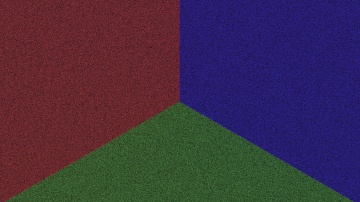
\includegraphics[width=\textwidth]{imgs/escena_3_planos}
        \caption{Render de los planos x=0, y=0 y z=0}
        \label{fig:render_planos_0}
    \end{subfigure}
    \caption{Planos}
\end{figure}

En la figura~\ref{fig:render_plano_x0} vemos el plano $x=0$ en verde, mientras que en la
figura~\ref{fig:render_planos_0} vemos los 3 planos $x=0$, $y=0$ y $z=0$ en rojo, verde y azul
respectivamente.

\subsection{Cajas} \label{subsec:cajas}

Las cajas las implementamos con 6 planos, cada uno representando a la cara correspondiente.
Para que la implementación sea simple, decidimos que las caras estarían alineadas a los ejes
cartesianos.
Para verificar si un rayo colisiona con la caja, recorremos cada cara y calculamos el punto en el
que el rayo y el plano se intersecan.
Si este punto pertenece a alguna cara de la caja, lo consideramos para calcular el punto final,
que sería el más cercano.
Si ningún punto pertenece a una cara de la caja, consideramos que no hay colisión.

Las cajas se definen por 2 vertices opuestos, el que tiene las coordenadas menores y el que tiene
las coordenadas mayores.
En la figura~\ref{fig:escena_caja_vertices} podemos ver una caja con un vértice rojo $P=(0,.1,0)$
y un vértice amarillo $Q=(1,1.1,1)$.

\begin{figure}[H]
    \centering
    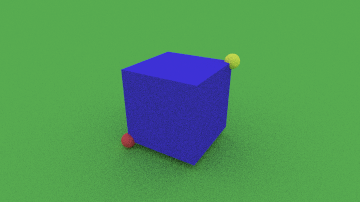
\includegraphics[width=.9\textwidth]{imgs/escena_caja_vertices}
    \caption{Render de una caja, indicando los vertices que lo identifican}
    \label{fig:escena_caja_vertices}
\end{figure}

\subsection{Triángulos} \label{subsec:triangulos}

Los triángulos los definimos con 3 vertices, $P_0, P_1$ y $P_2$.
Para calcular la intersección con un rayo, primero calculamos la intersección con el plano que
contiene al triangulo y luego verificamos si este punto $P$ se encuentra dentro del triangulo.
Para hacer esto, calculamos las normales de los triángulos $P_0 P_1 P$, $P_1 P_2 P$ y $P_2 P_0 P$.
Si estas normales apuntan hacia el mismo lado que la normal del triangulo original, entonces el
punto $P$ se encuentra dentro.

\begin{figure}[H]
    \centering
    
\includegraphics[width=.9\textwidth]{imgs/escena_triangulo}
    \caption{Render de un triángulo}
    \label{fig:escena_triangulo}
\end{figure}

En la figura~\ref{fig:escena_triangulo} vemos un triangulo de vertices $(1,0,0)$, $(0,1,0)$ y $
(0,0,1)$.

\section{Estructuras} \label{sec:estructuras}

Además, de los objetos mencionados, agregamos 3 estructuras adicionales para facilitar el
renderizado de objetos más complejos:

\begin{itemize}
    \item Lista de objetos
    \item Malla de triángulos
    \item KD Tree
\end{itemize}

A continuación explicamos brevemente la implementación de cada uno.
\subsection{Lista de objetos} \label{subsec:lista_objetos}

Tiene una implementación muy directa, ya que como su nombre indica, solo almacena una lista
de objetos (básicos u otras estructuras).
La colisión de un rayo contra este se calcula como el punto más cercano de colisión entre el rayo y
alguno de los objetos que almacena, si es que hubiese colisión.

Es una estructura de utilidad para facilitar el renderizado de escenas o para crear otras
estructuras más complejas, como las que veremos a continuación.

\subsection{Malla de Triángulos} \label{subsec:malla_triangulos}

Las mallas de triángulos por lo general consisten de miles de objetos, por lo que la
implementación de esta estructura toma como parámetro un archivo en el que se definen los mismos.
El archivo consiste de lineas de tipo vértice, en el que se indican las coordenadas de cada
vértice, y de tipo cara, en el que se indican que vertices componen a cada triangulo.
Dejando de lado esa diferencia, la implementación es prácticamente la misma que la lista de objetos,
solo que almacena triángulos.

En la figura~\ref{fig:escena_malla_pato} podemos ver el render del modelo de un pato.

\begin{figure}[H]
    \centering
    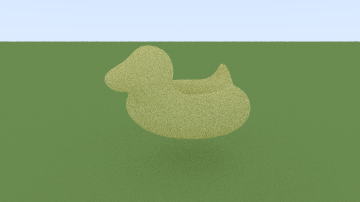
\includegraphics[width=.9\textwidth]{imgs/escena_malla_pato}
    \caption{Render de una malla de triángulos.}
    \label{fig:escena_malla_pato}
\end{figure}

Sin embargo, debido a la sencillez de la implementación de la lista de objetos, esta estructura
resulta muy lenta ya que se debe recorrer los miles de triángulos uno por uno para detectar
colisiones.
Para poder mitigar el tiempo de procesamiento, utilizamos la siguiente estructura para calcular
menos colisiones, el KD Tree.

\subsection{KD Tree} \label{subsec:kd_tree}

El problema que tiene la implementación anterior es que la complejidad para saber si un rayo
colisiona con algún triángulo de la malla crece con la cantidad de objetos en la lista.

Los \textit{axis-aligned bounding boxes} (AABB) son estructuras que mejoran la complejidad
dependiendo del tipo (Octree, BPS Tree, KD Tree, etc.).
Logran esto dividiendo el espacio en partes iguales, y encerrando cada parte en una caja que
contenga todos sus objetos.
Luego cada partición del espacio se divide de la misma forma, creando así una jerarquía de cajas
asociada a cada nodo de un árbol.
La raíz del árbol representa la caja más grande que contiene todos los objetos, y los nodos hijos
están asociados a cada partición del espacio, con sus respectivas cajas.

El \textit{KD Tree} es una estructura AABB en el que en cada paso de la división del espacio, se
hace un único corte en el eje donde la longitud de la caja es mayor.
Esto significa que el árbol resultante es un árbol binario, ya que cada espacio se divide en 2.

Esta nueva estructura puede recibe como parámetro una lista de objetos y un entero indicando
cuantos elementos debe tener las hojas del árbol.
Luego se procede a dividir el espacio hasta llegar a nodos que contengan como máximo la cantidad
indicada.
De esta forma, si se especifica como lista de objetos una malla de 16000 triángulos y como cantidad
máxima 500 objetos, el espacio se divide hasta llegar a un árbol de altura 6 con 32 hojas, cada una
con 500 triángulos.

Esta estructura nos permitió acelerar el renderizado tanto de las mallas de triángulos, como de
escenas complejas que cuentan con muchos objetos.

\newpage
\section{Resultados y Conclusión} \label{sec:conclusion}

En la figura~\ref{fig:escena_final} podemos observar un render con todos los objetos y
estructuras mencionadas en este trabajo.

\begin{figure}[H]
    \centering
    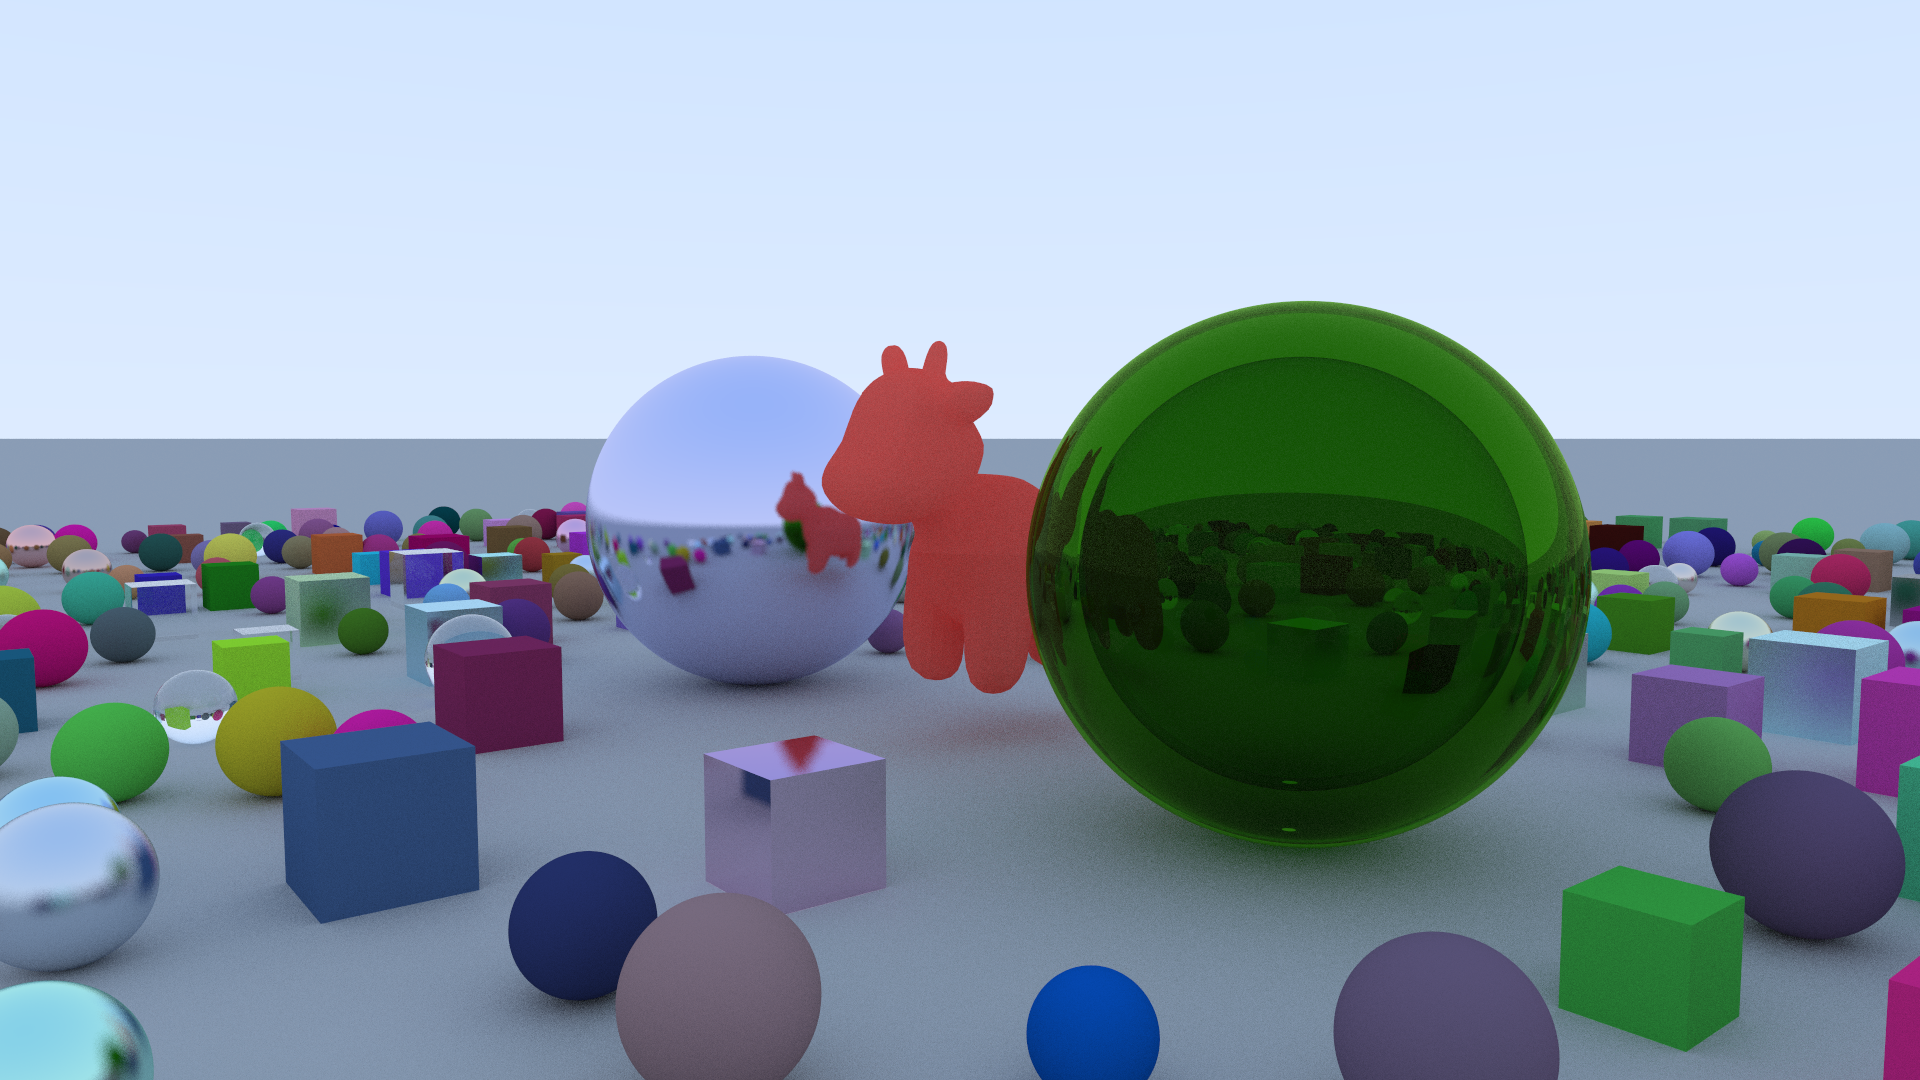
\includegraphics[width=.9\textwidth]{imgs/escena_final}
    \caption{Render de una malla de triángulos.}
    \label{fig:escena_final}
\end{figure}

Luego de ver en detalle dos técnicas de renderizado, una basada en \textit{object-order
rendering} (rasterización), y otra en \textit{image-order rendering} (ray tracing), las
diferencias son claras.

La rasterización cuenta con algoritmos que al día de hoy han sido optimizados a tal punto que
existe todo un pipeline dentro de la mayoría de las tarjetas gráficas.
Es necesario conocer este pipeline y la librería correspondiente para interactuar con el mismo, pero
su optimización resulta en renders de buena calidad en muy poco tiempo.

Por otro lado, los algoritmos de ray tracing suelen ser más intuitivos en cuanto a la idea
general y su implementación, y no requieren (en principio) de conocimientos de ninguna librería.
Si bien en la actualidad surgen nuevas tarjetas gráficas que incluyen unidades para realizar la
intersección de los rayos de manera optimizada, la realidad es que sin estos recursos el ray
tracing resulta lento en comparación a la rasterización.
Sin embargo, la calidad de las imágenes resultantes son claramente superiores y más realistas.

El futuro del ray tracing y su aplicación tanto en videojuegos como en producciones audiovisuales
resulta muy prometedor.
Las nuevas tarjetas gráficas capaces de realizar ray tracing en tiempo real permitirán que esta
rama de la computación gráfica avance a pasos agigantados y que la calidad del
contenido multimedia que producimos y consumimos crezca de manera acorde.

\end{document}
